\chapter{Manual de usuario}
\label{cap:Manual de usuario}

\section{Permisos}

Para el correcto funcionamiento de la aplicación es necesario que el usuario de permisos a la aplicación para poder acceder tanto a la cámara, como a las imágenes del dispositivo.\\

Al iniciar la aplicación se nos pedirá permiso para acceder al contenido del teléfono, ya que es en ese instante, cuando se inicia la aplicación, el momento en el que se listan todas las imágenes del dispositivo.

\begin{figure}[H] %con el [H] le obligamos a situar aquí la figura
\centering
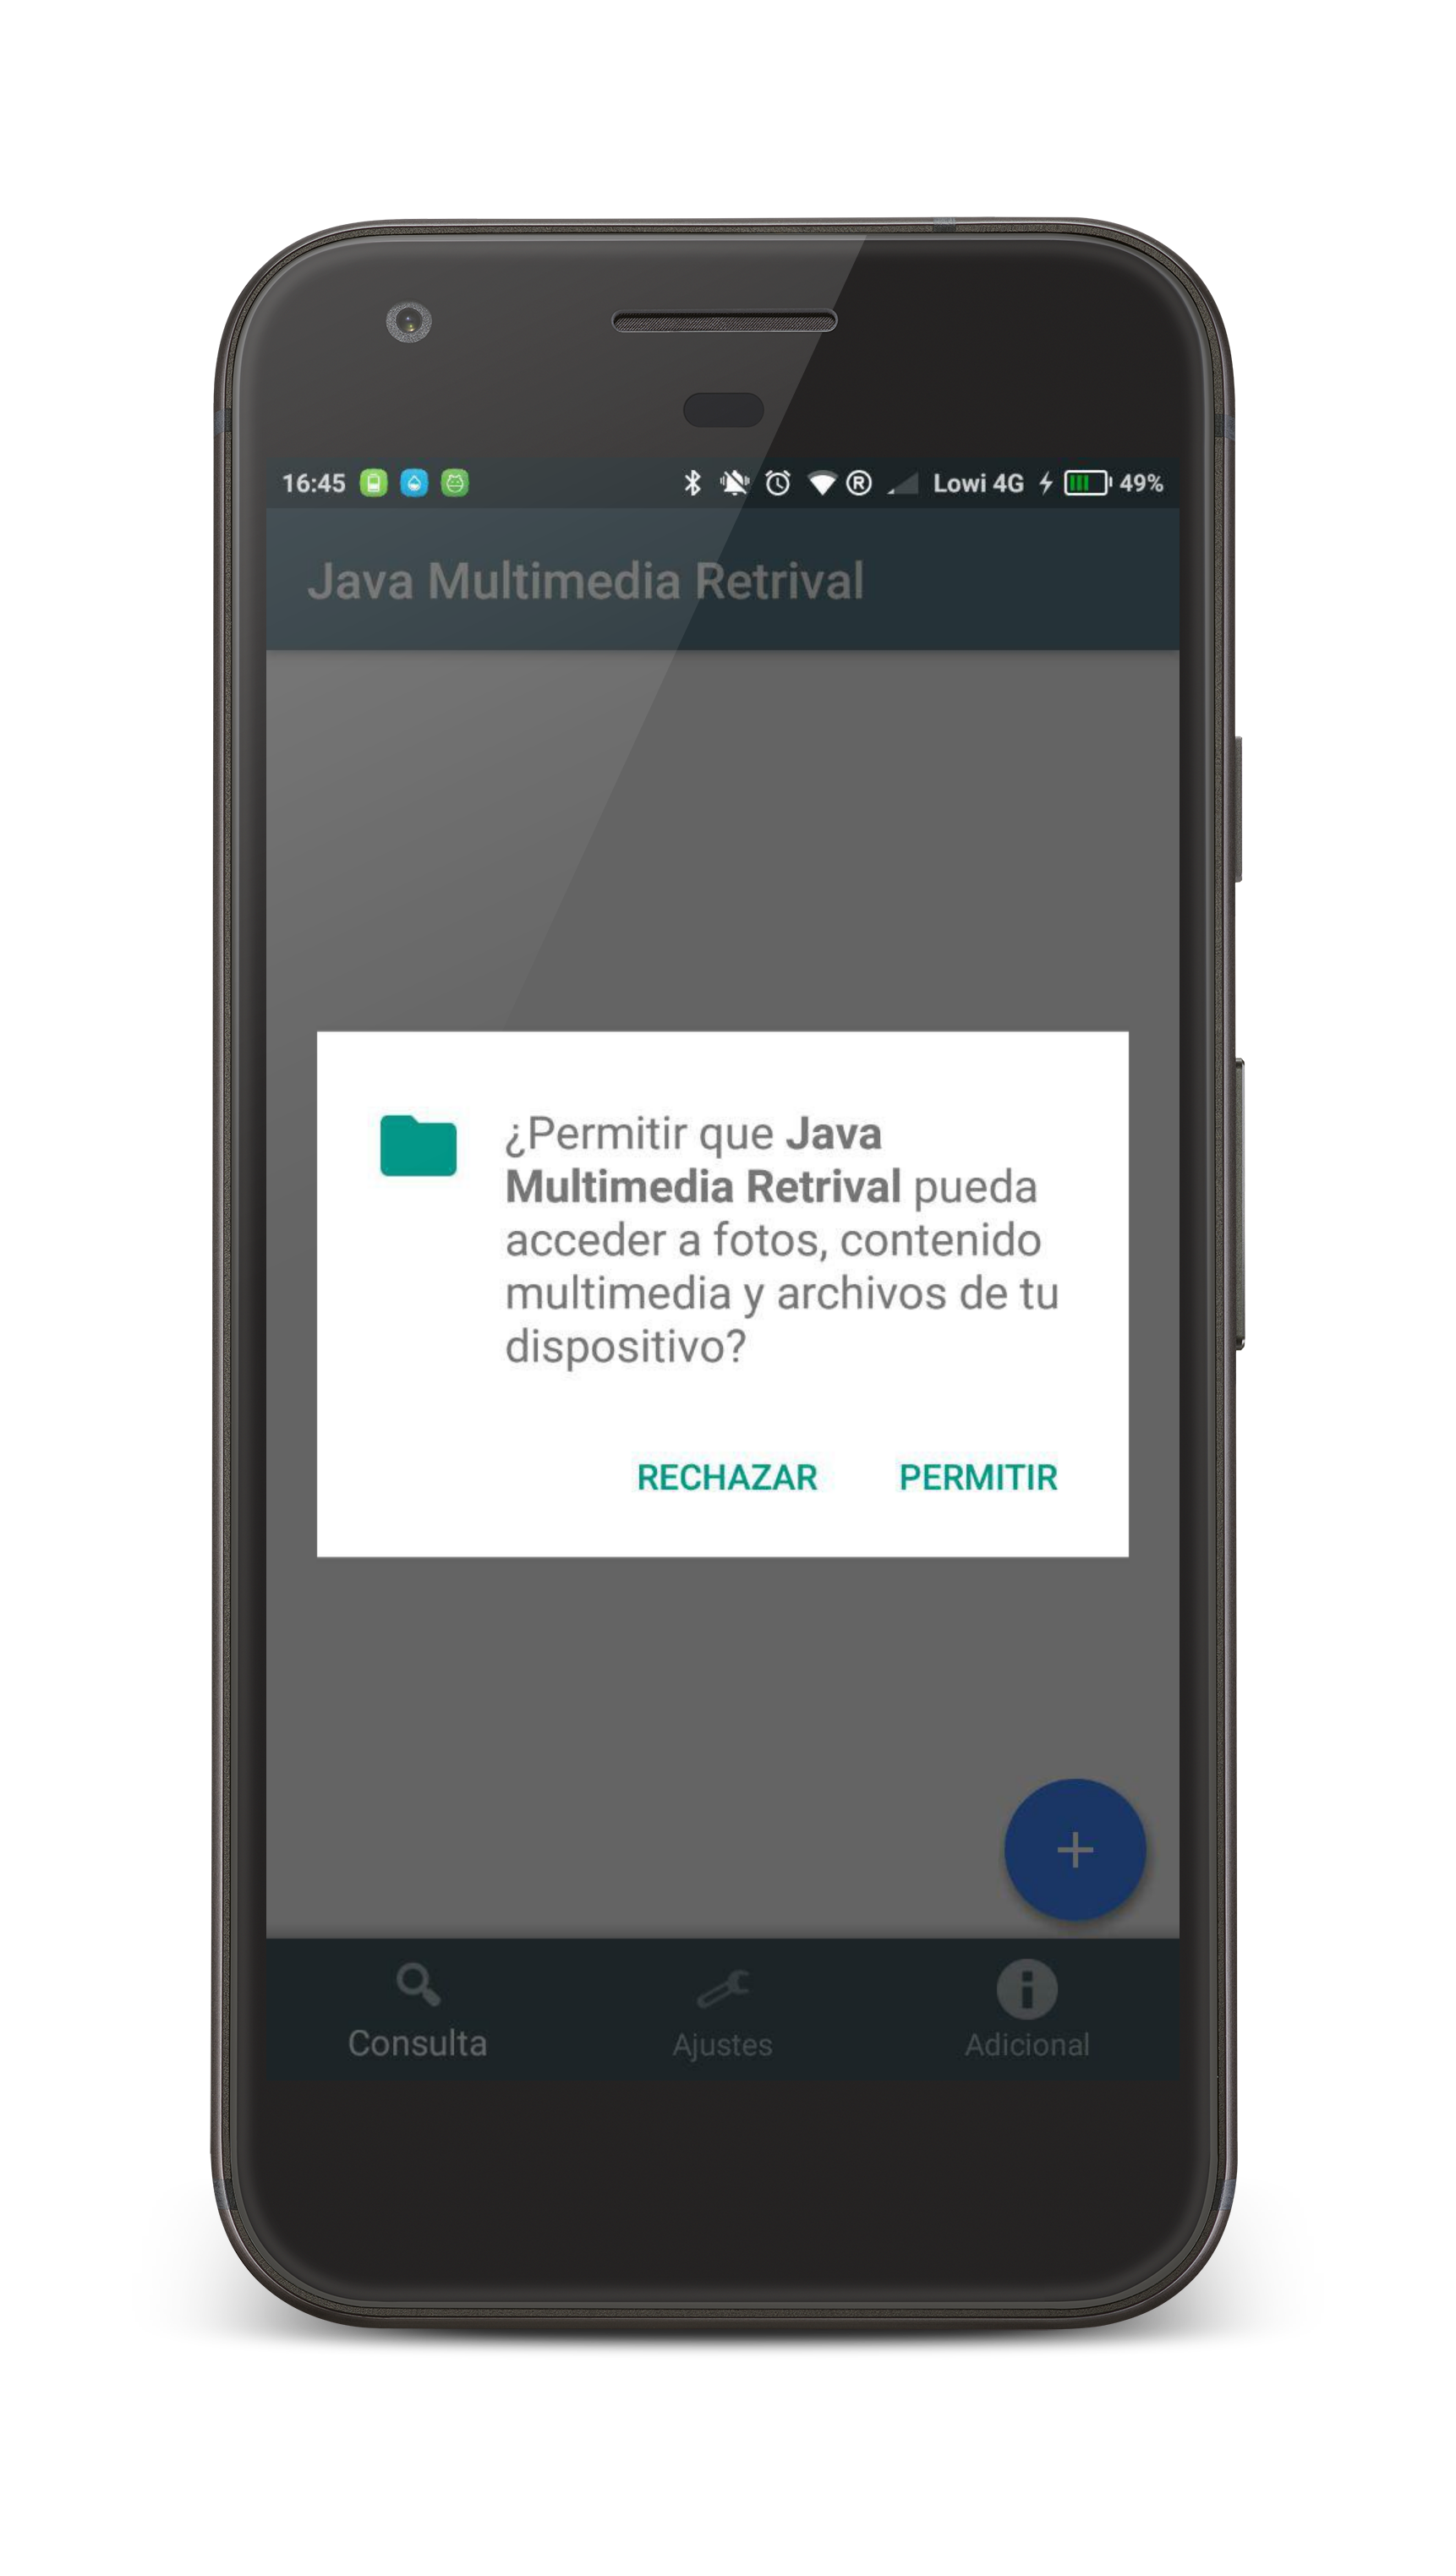
\includegraphics[scale=0.15]{imagenes/permisos1.png}  %el parámetro scale permite agrandar o achicar la imagen. En el nombre de archivo puede especificar directorios
\label{permisos1.png}
\caption{Permisos aplicación 1}
\end{figure}

En caso de no conceder el permiso, cuando intentemos acceder al recurso otra vez, galería o cámara, se nos volverá a preguntar. Una vez aceptado, ya podemos acceder a los recursos requeridos sin ningún tipo de problema.

\begin{figure}[H] %con el [H] le obligamos a situar aquí la figura
\centering
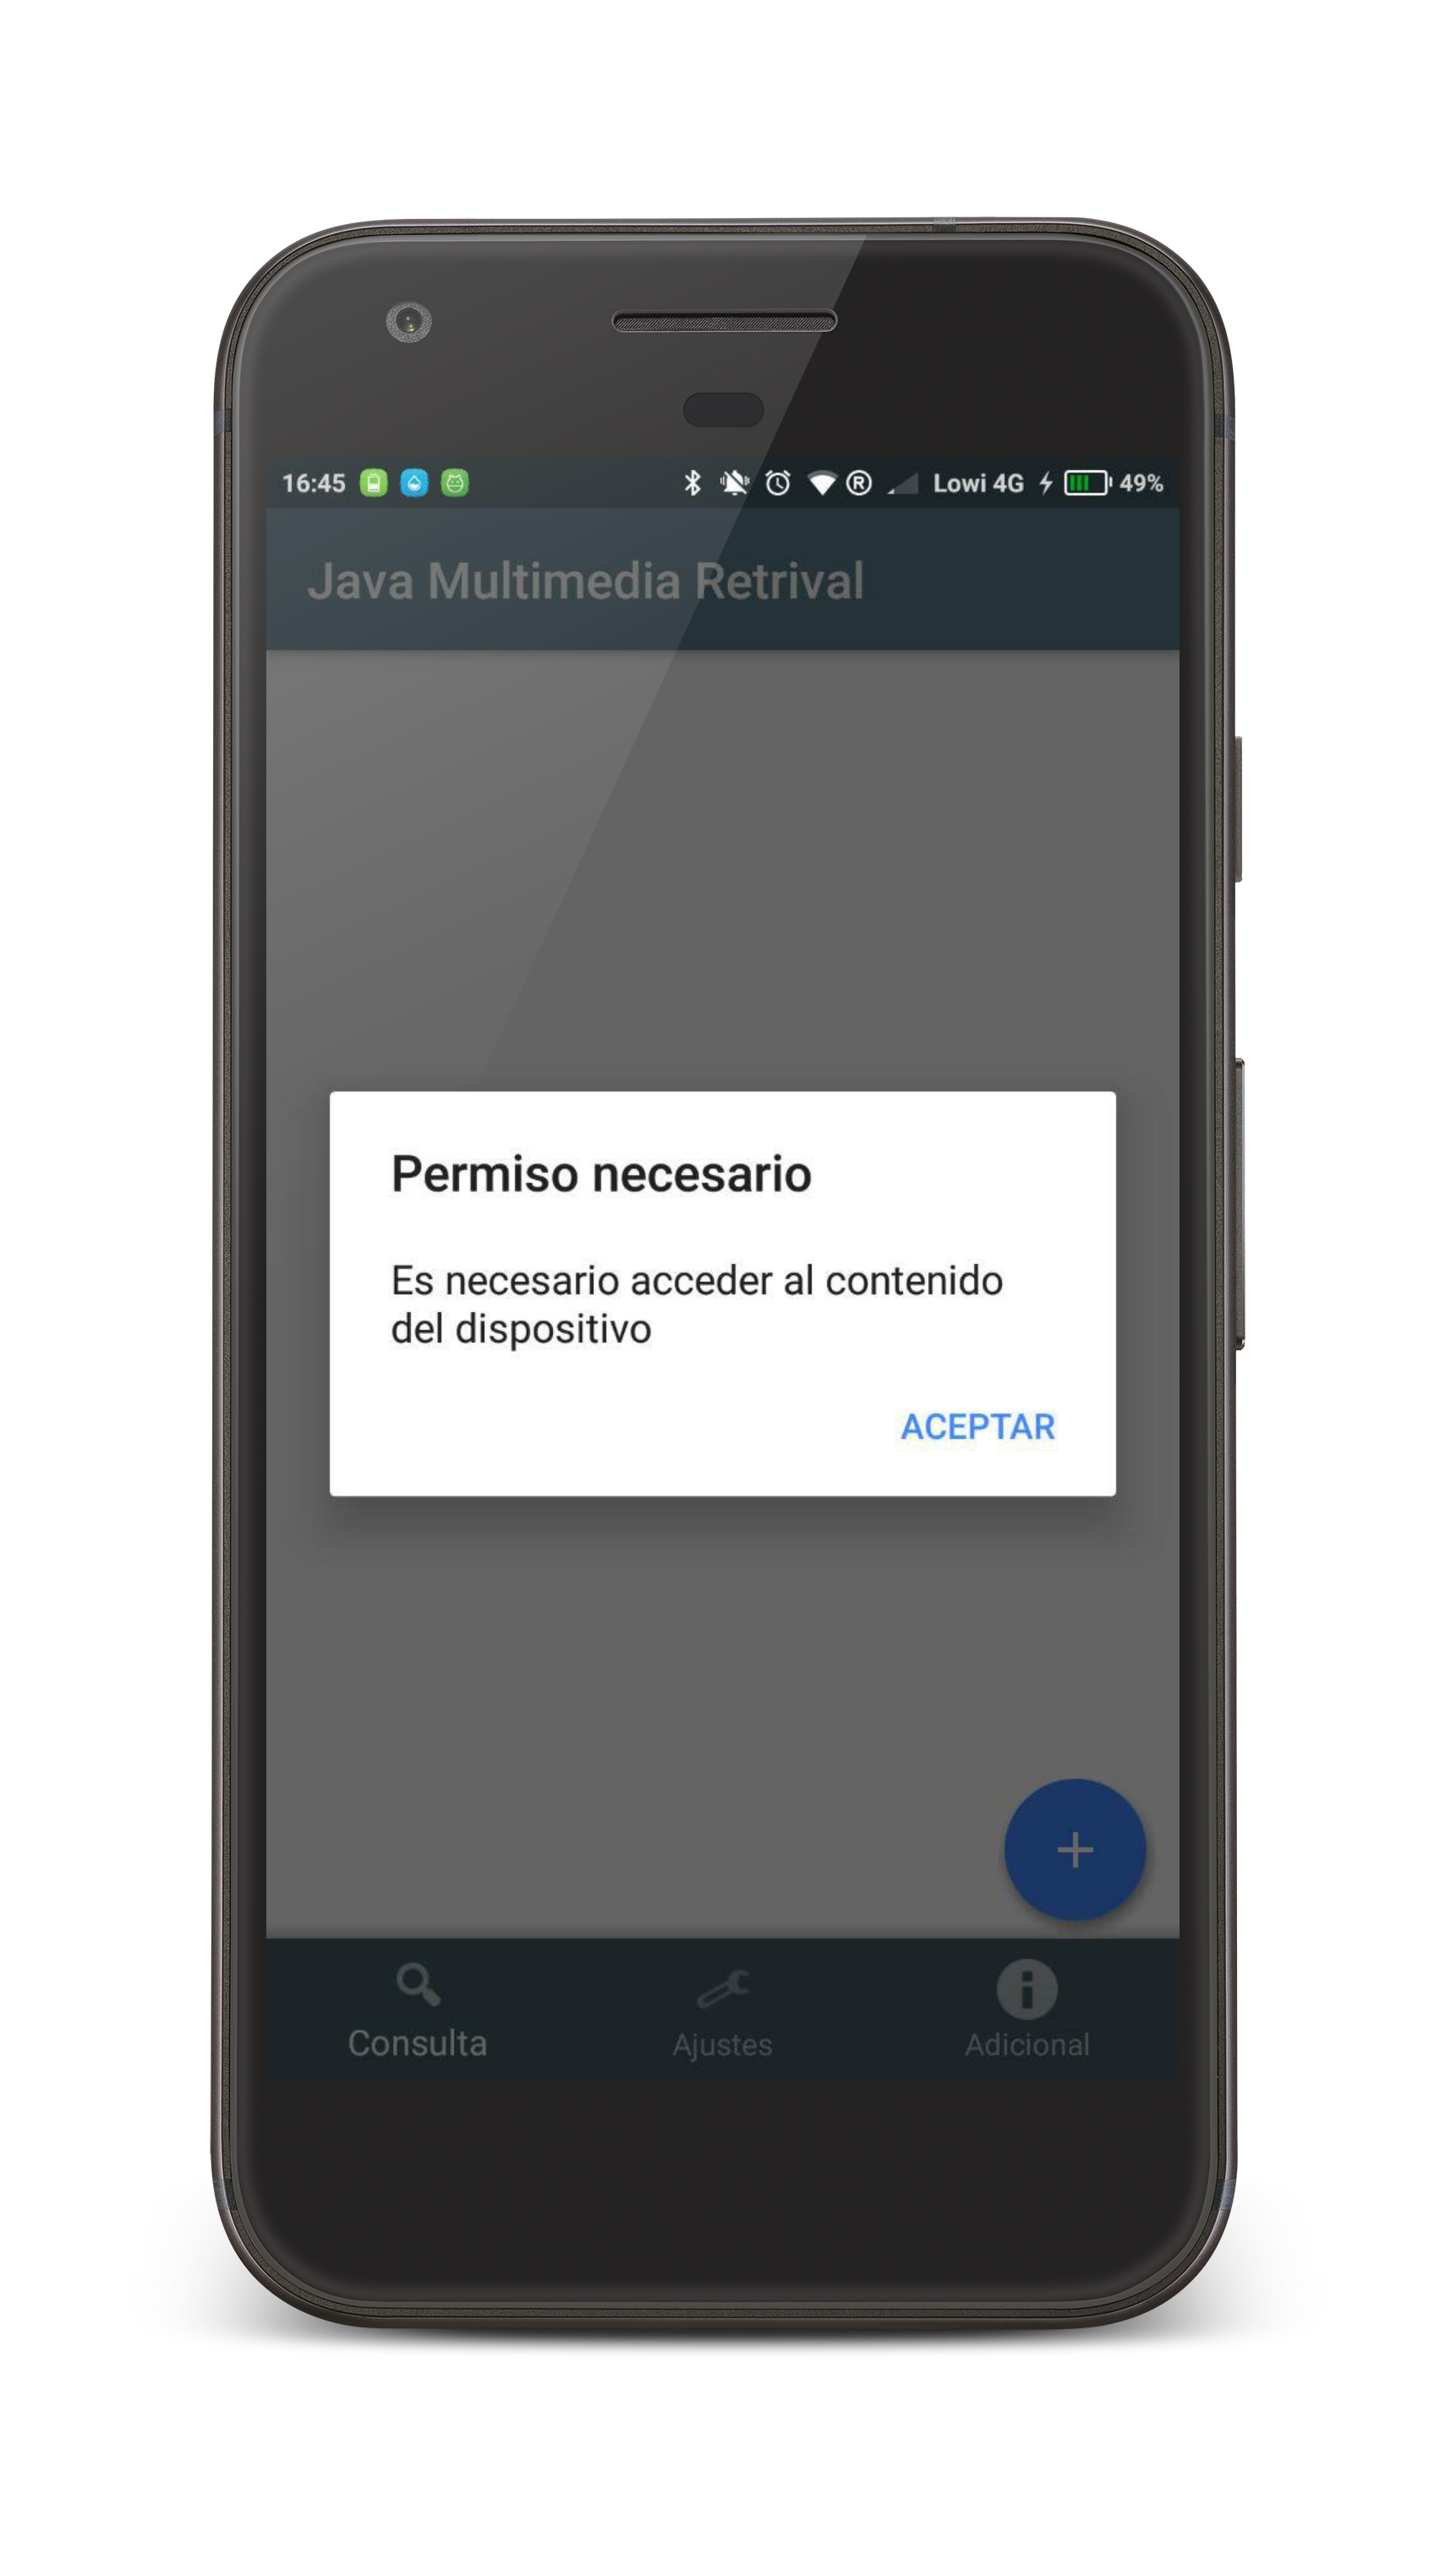
\includegraphics[scale=0.15]{imagenes/permisos2.png}  %el parámetro scale permite agrandar o achicar la imagen. En el nombre de archivo puede especificar directorios
\label{permisos2.png}
\caption{Permisos aplicación 2}
\end{figure}

\section{Navegación}

Para moverse a través de la aplicación, se dispone de un menú inferior con 3 elementos o ítems, cada uno representa una pantalla distinta. Por defecto la pantalla inicial es la correspondiente a la de consulta, ya que es el corazón de la aplicación.\\

Se pueden pulsar cada uno de los ítems para cambiar a su pantalla correspondiente. Cada pantalla tiene elementos propios y no son compartidos. Por ejemplo, el \textit{floating button} azul solo aparece en la pantalla de consulta.\\

\begin{figure}[H] %con el [H] le obligamos a situar aquí la figura
\centering
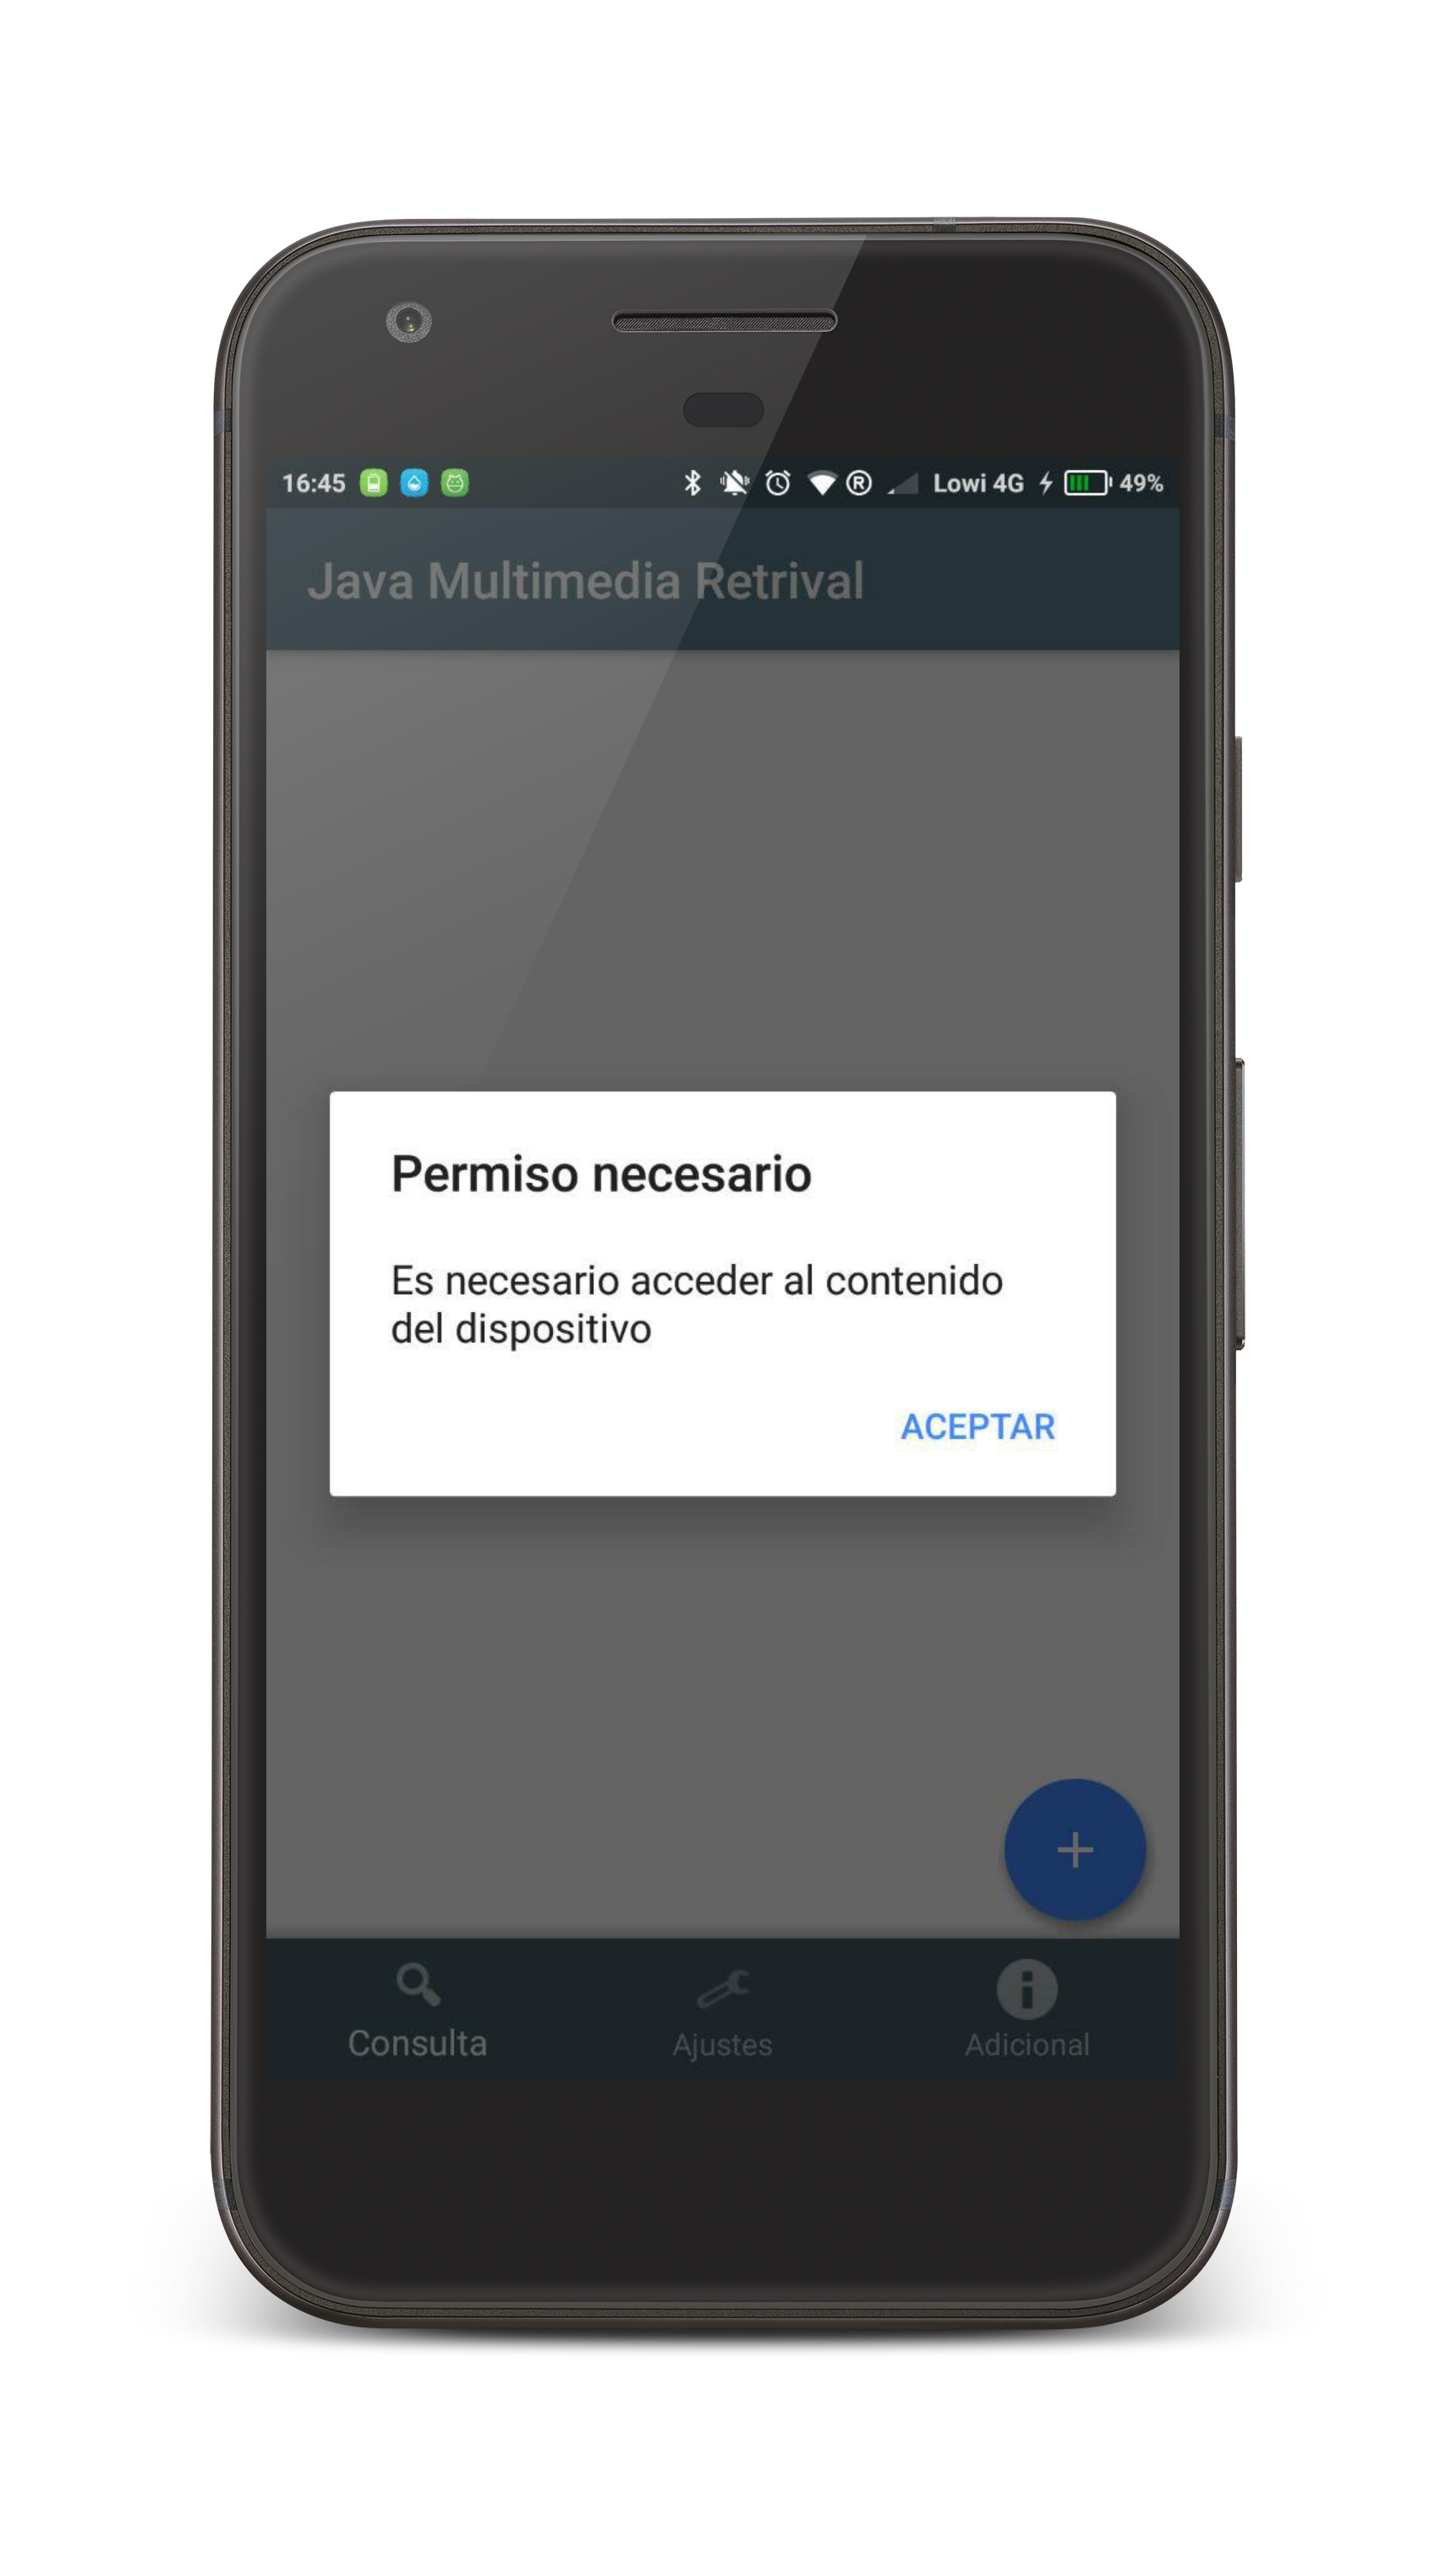
\includegraphics[scale=0.15]{imagenes/permisos2.png}  %el parámetro scale permite agrandar o achicar la imagen. En el nombre de archivo puede especificar directorios
\label{permisos2.png}
\caption{Ejemplo de navegación 1}
\end{figure}

\begin{figure}[H] %con el [H] le obligamos a situar aquí la figura
\centering
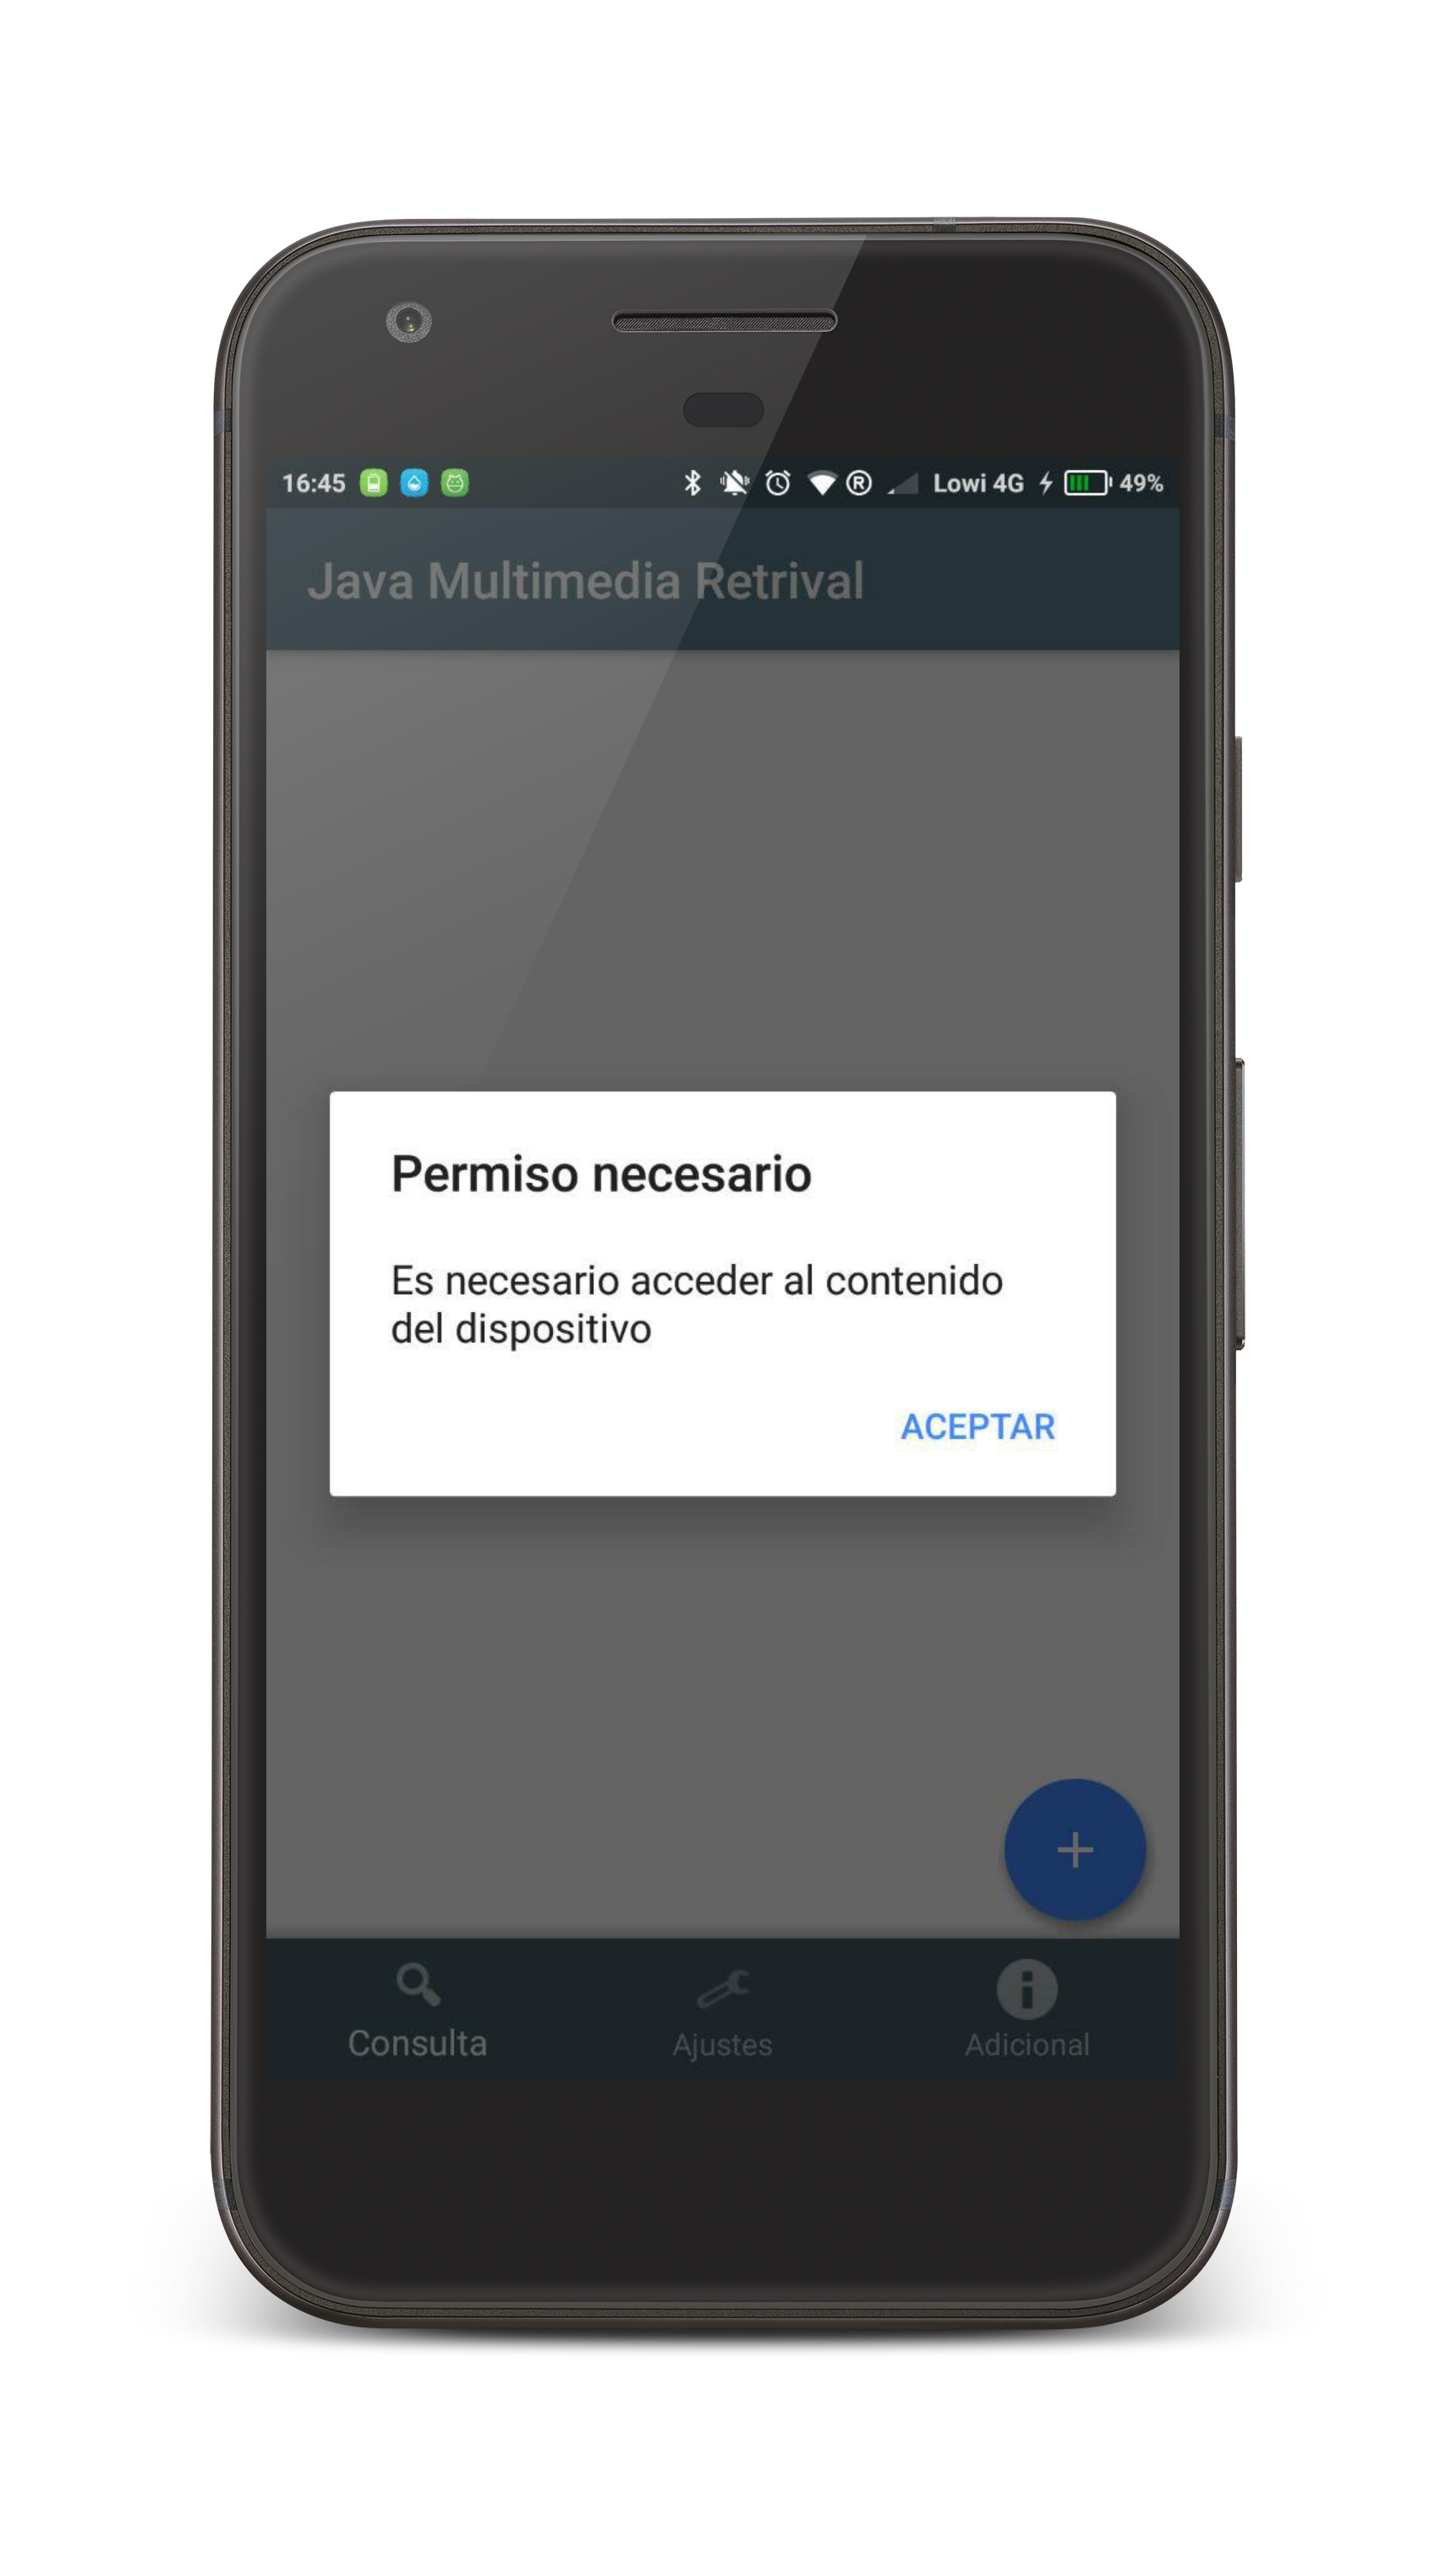
\includegraphics[scale=0.15]{imagenes/permisos2.png}  %el parámetro scale permite agrandar o achicar la imagen. En el nombre de archivo puede especificar directorios
\label{permisos2.png}
\caption{Permisos navegación 2}
\end{figure}

\section{Consulta}

Para realizar la consulta disponemos de dos opciones, elegir una imagen desde la cámara o desde la galería. Estas opciones aparecen al pulsar sobre el botón flotante. Una vez elegida una, se lanzará la cámara, pudiendo elegir la trasera o delantera, o la galería, mediante la cual podremos acceder a cualquier imagen del dispositivo. Cuando sea seleccionada, esta aparecerá en la parte superior de la aplicación.

\begin{figure}[H] %con el [H] le obligamos a situar aquí la figura
\centering
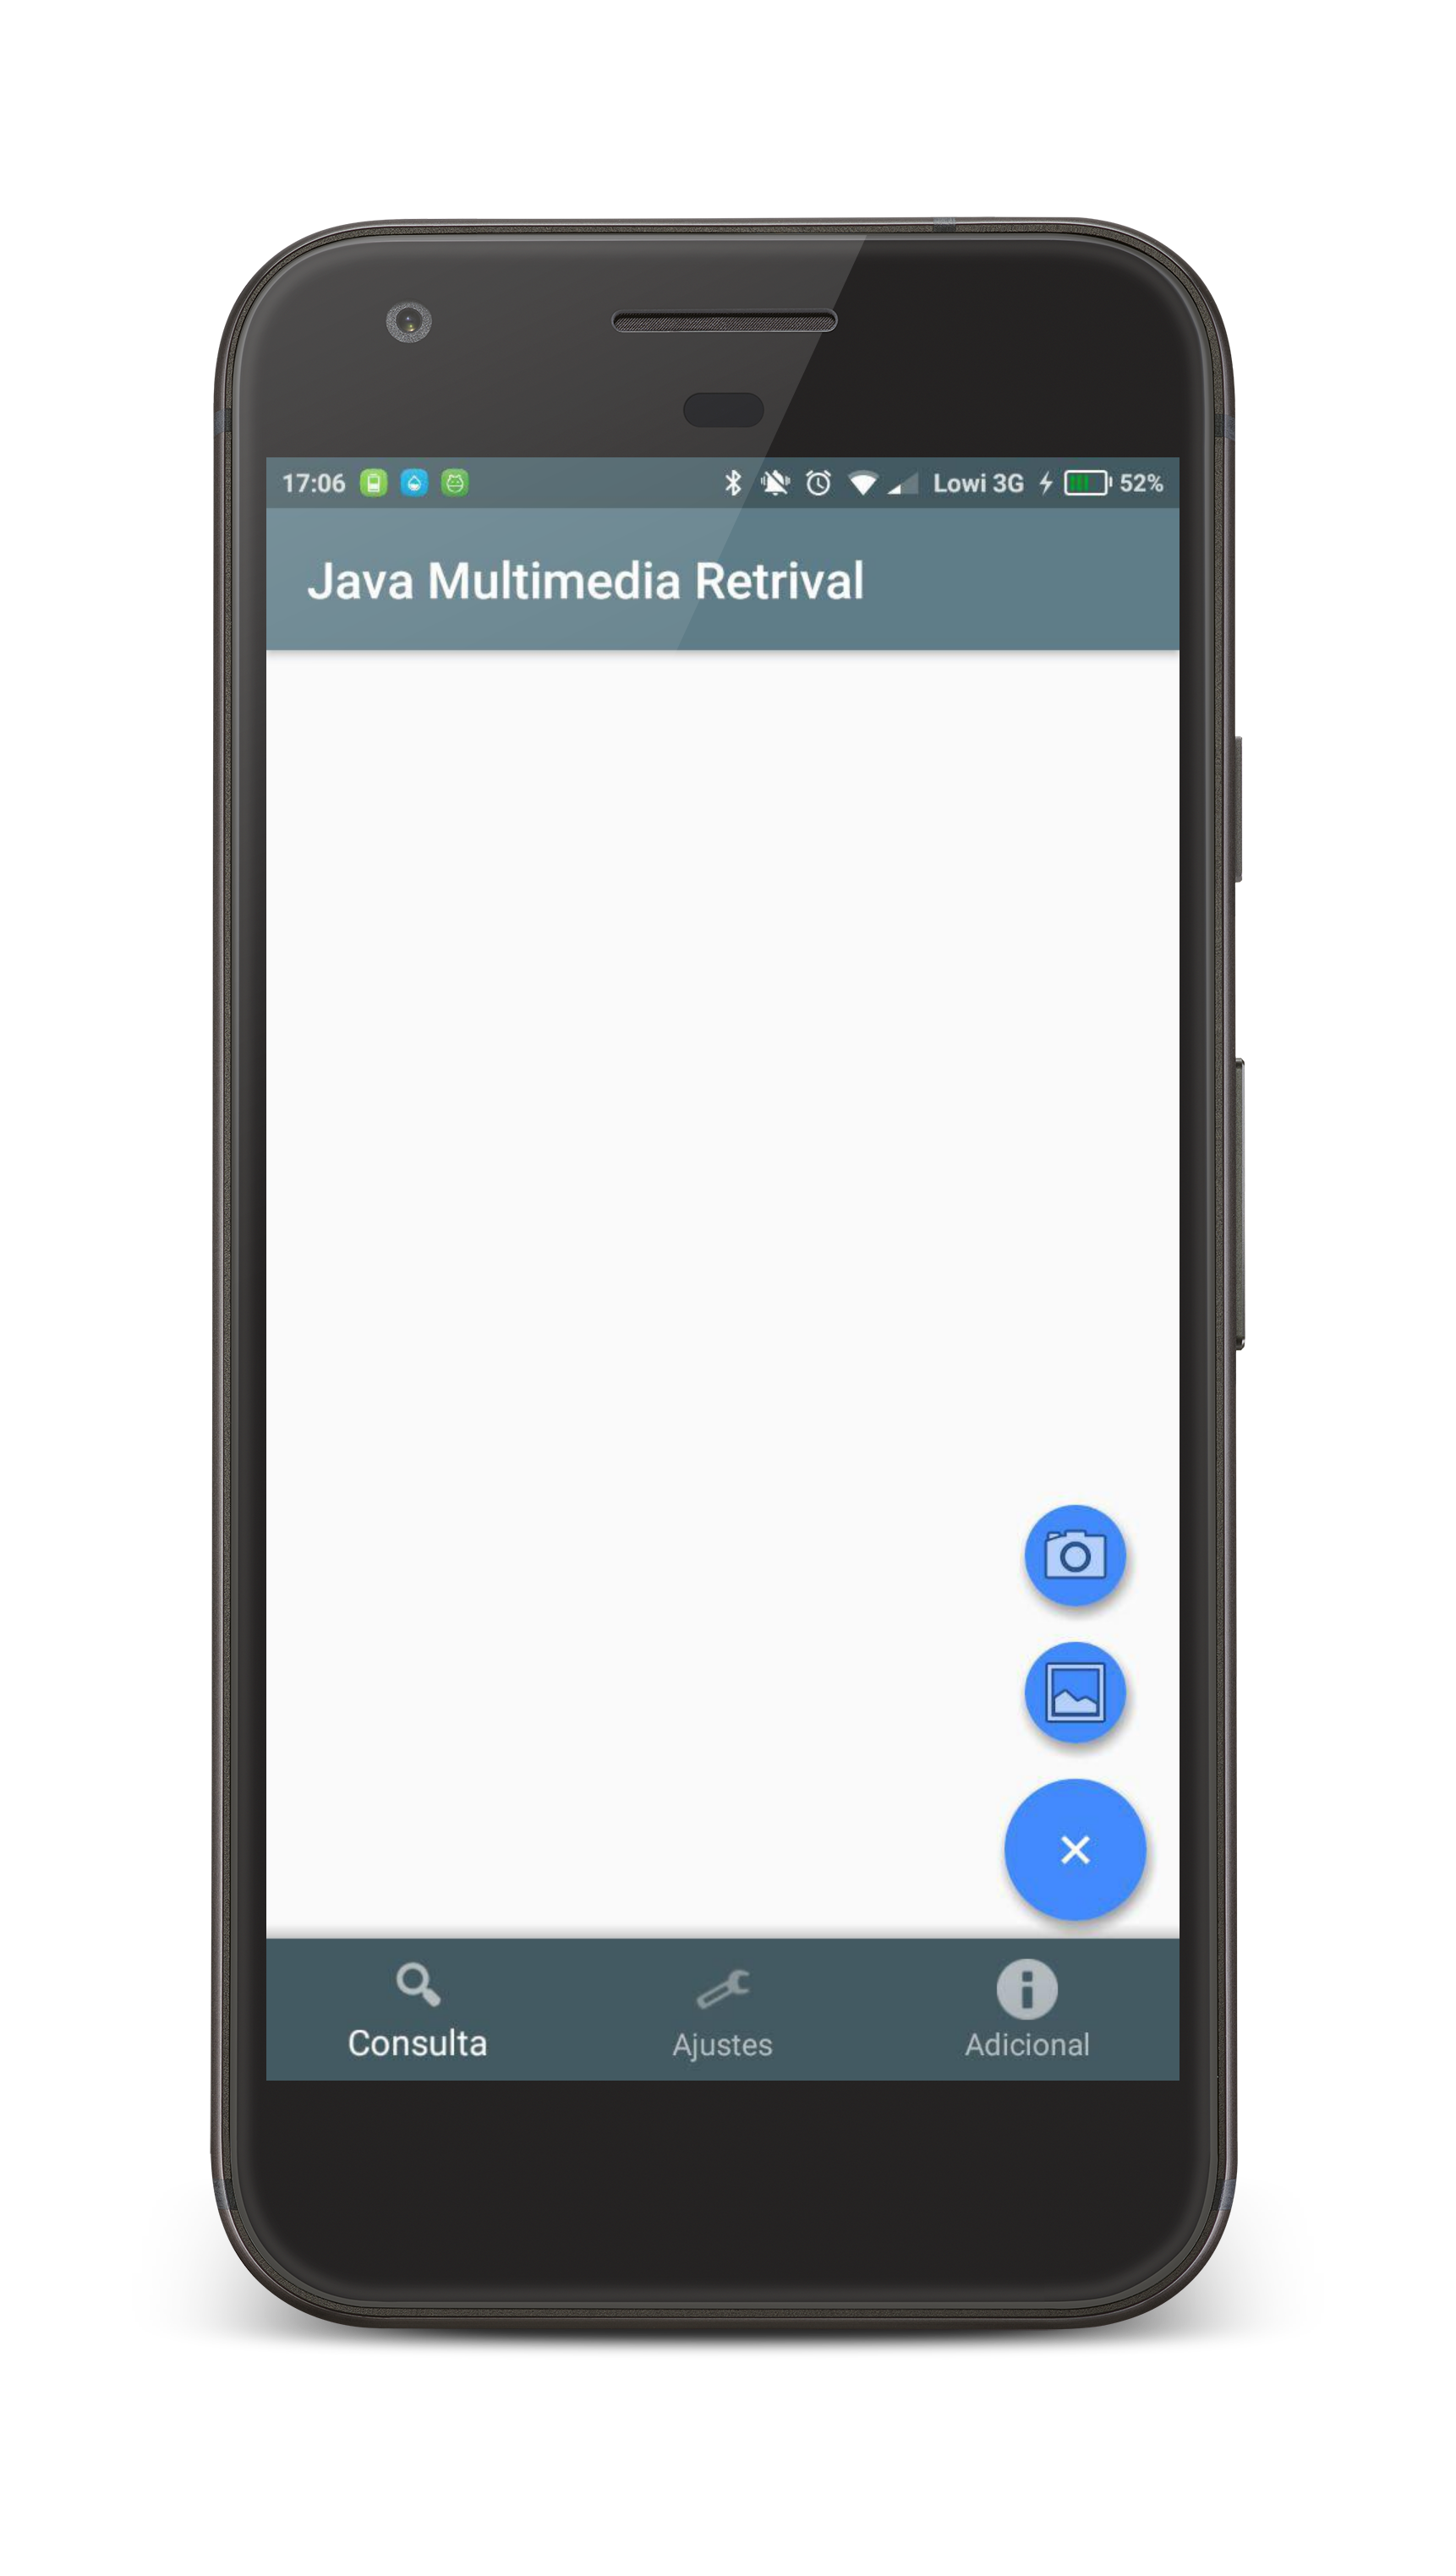
\includegraphics[scale=0.15]{imagenes/hacerconsulta.png}  %el parámetro scale permite agrandar o achicar la imagen. En el nombre de archivo puede especificar directorios
\label{hacerconsulta.png}
\caption{Realizar consulta}
\end{figure}

\section{Ajustes}

En este apartado vamos a hablar de los ajustes que puede realizar el usuario sobre las consultas.\\

\begin{figure}[H] %con el [H] le obligamos a situar aquí la figura
\centering
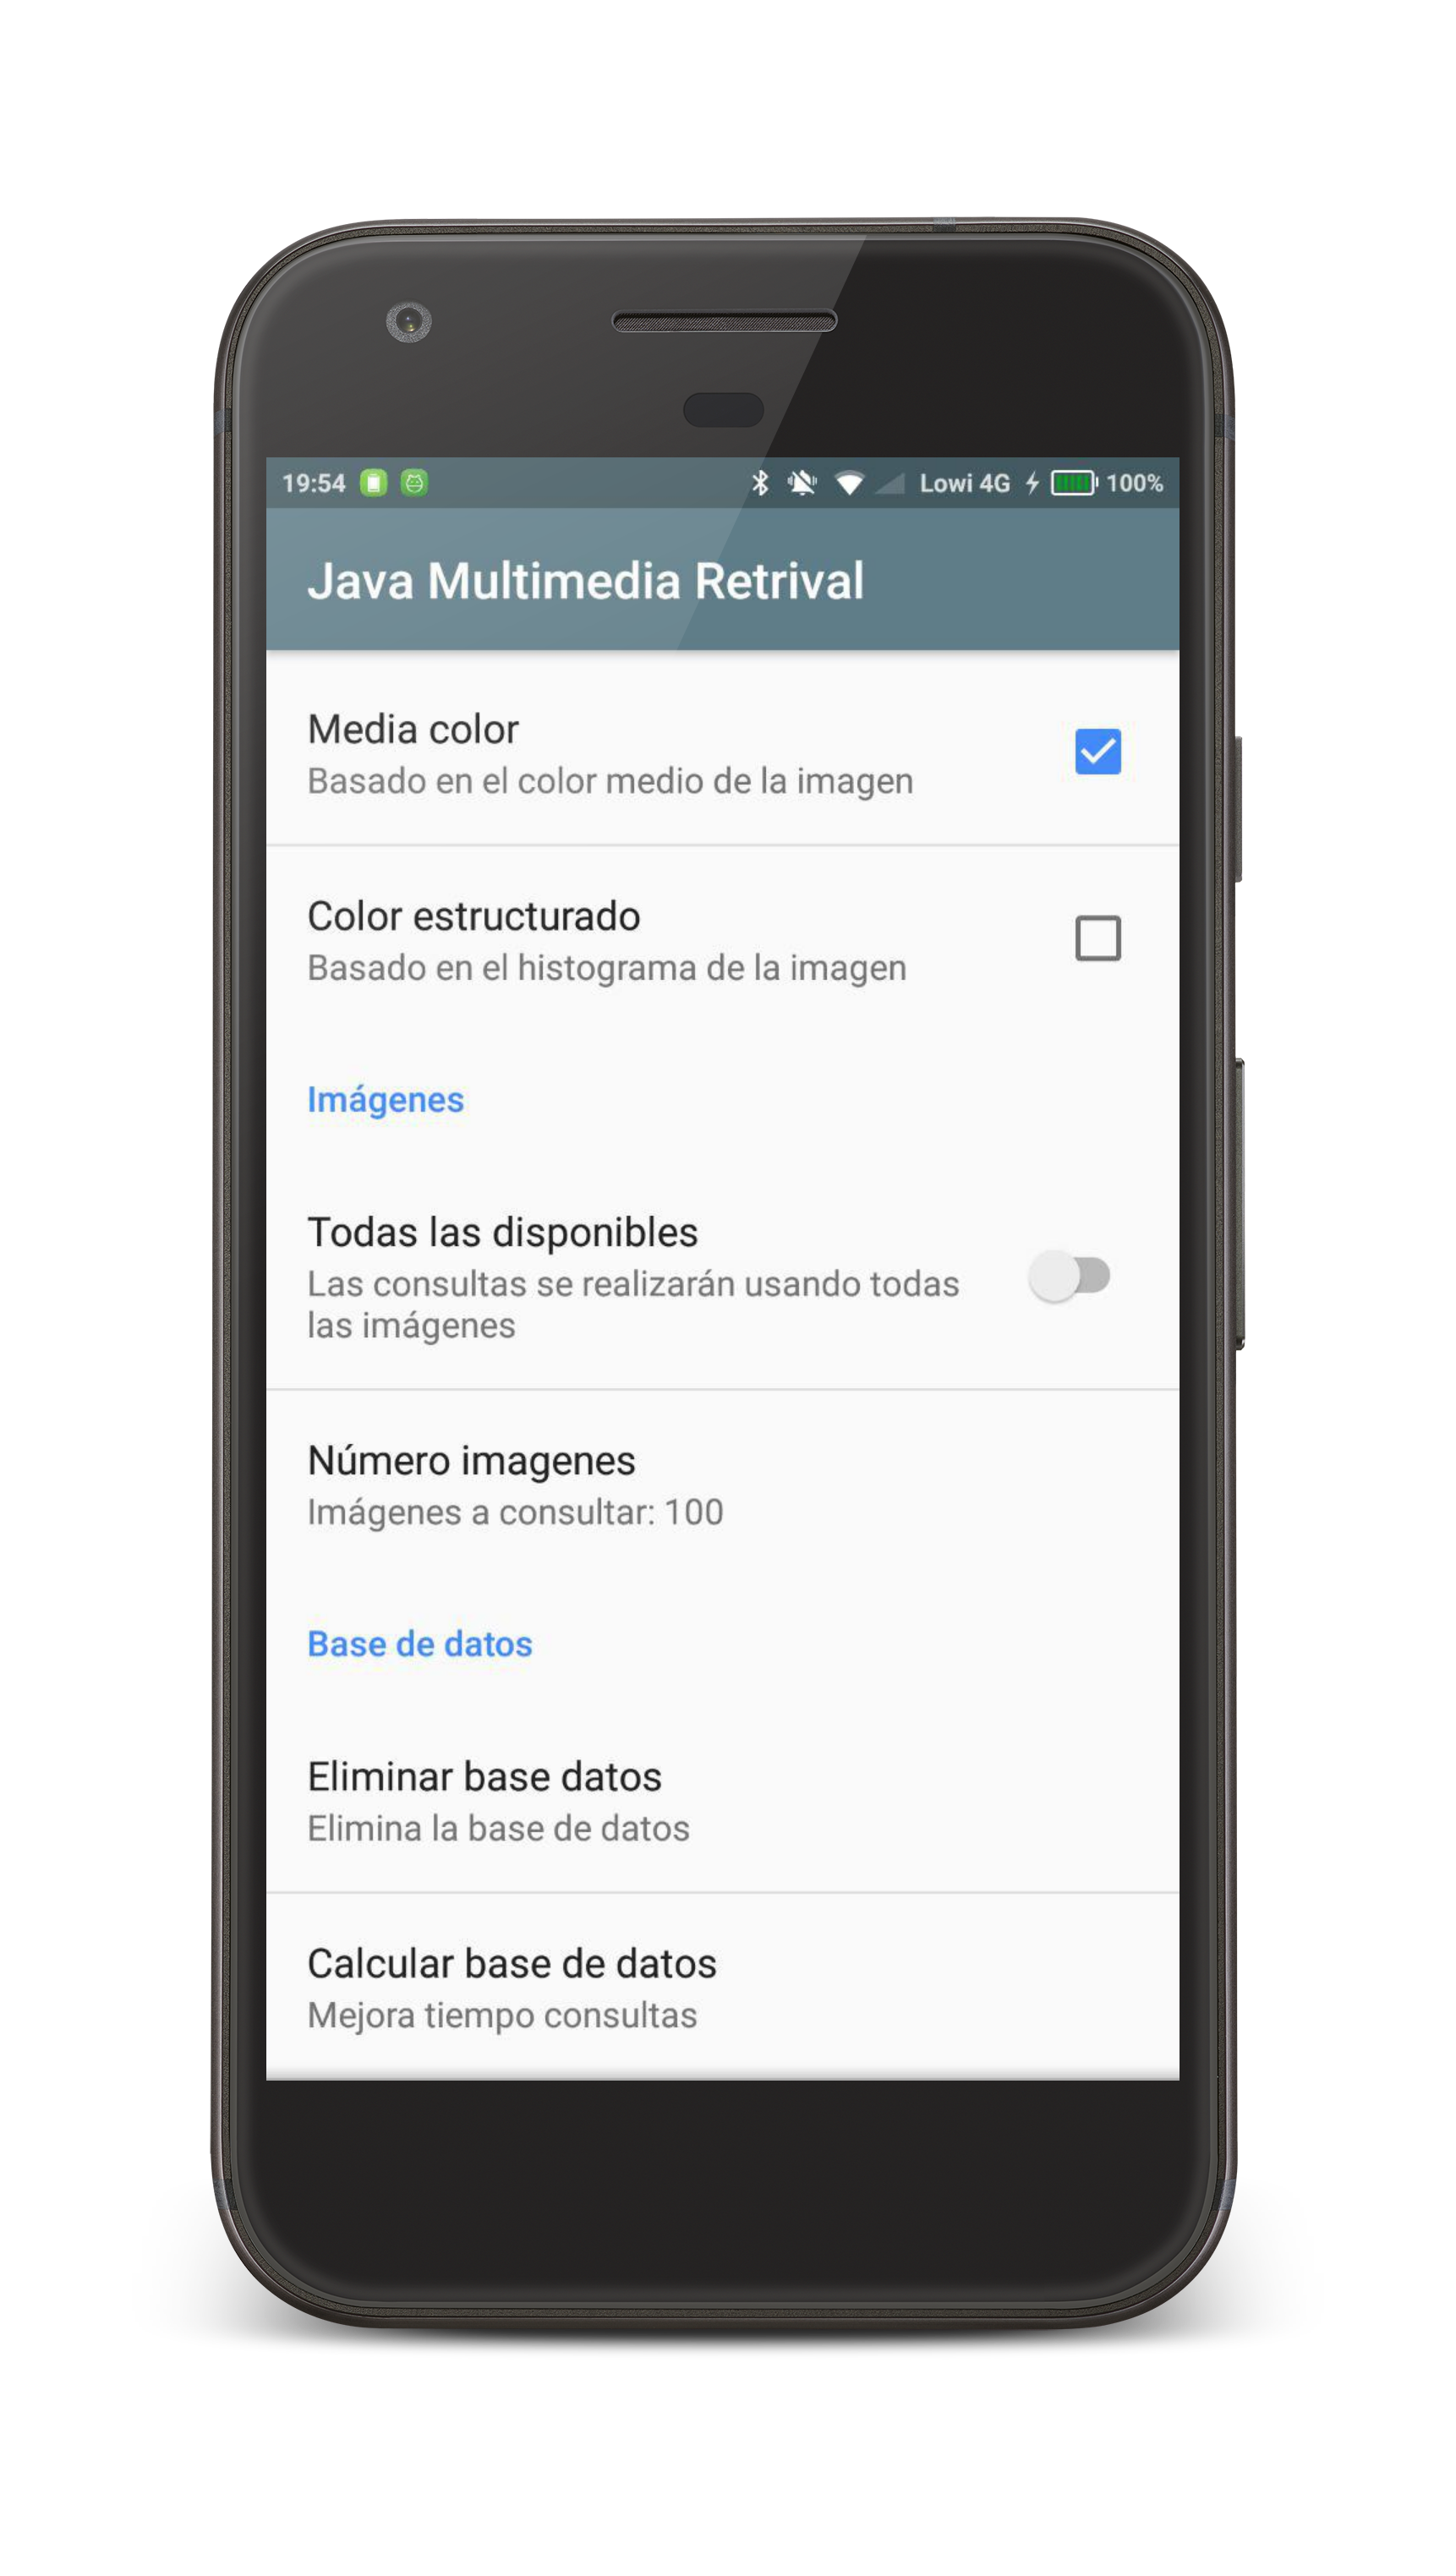
\includegraphics[scale=0.15]{imagenes/ajustes.png}  %el parámetro scale permite agrandar o achicar la imagen. En el nombre de archivo puede especificar directorios
\label{ajustes.png}
\caption{Pantalla ajustes}
\end{figure}

Podríamos hablar de tres secciones:

\subsection{Descriptores}

Aquí podemos encontrar los descriptores de los que dispone la aplicación. El usuario puede elegir uno libremente, pero solo un descriptor puede ser elegido a la vez.

\begin{figure}[H] %con el [H] le obligamos a situar aquí la figura
\centering
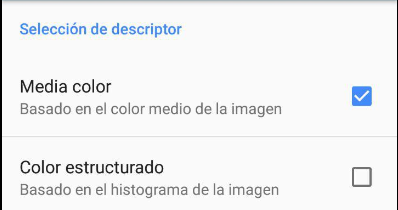
\includegraphics[scale=0.5]{imagenes/ajustesdescriptor.png}  %el parámetro scale permite agrandar o achicar la imagen. En el nombre de archivo puede especificar directorios
\label{ajustesdescriptor.png}
\caption{Pantalla ajustes. Sección descriptores}
\end{figure}

\subsection{Imágenes}

En este apartado el usuario puede elegir el número de imágenes totales sobre las cuales quiere realizar la consulta. Tiene dos opciones, introducir dicho valor manualmente o seleccionar todas las del dispositivo. Este valor también se usa en el caso de querer calcular la base de datos, cosa que veremos a continuación.

\begin{figure}[H] %con el [H] le obligamos a situar aquí la figura
\centering
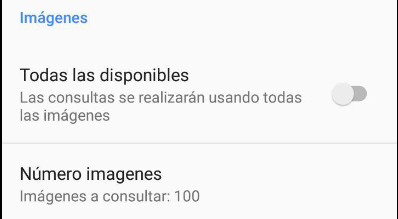
\includegraphics[scale=0.5]{imagenes/ajustesimagenes.png}  %el parámetro scale permite agrandar o achicar la imagen. En el nombre de archivo puede especificar directorios
\label{ajustesimagenes.png}
\caption{Pantalla ajustes. Sección imágenes}
\end{figure}

\subsection{Base de datos}

Aquí el usuario puede precalcular la base de datos, de esta manera al realizar la consulta no se calcularán nada, simplemente se obtendrán los valores de la base de datos. Este precálculo se realiza para todos los descriptores del sistema.\\

Por otro lado, puede borrar la base de datos si así lo desea. Realizando se calcularán los valores de la base de datos durante la consulta.

\begin{figure}[H] %con el [H] le obligamos a situar aquí la figura
\centering
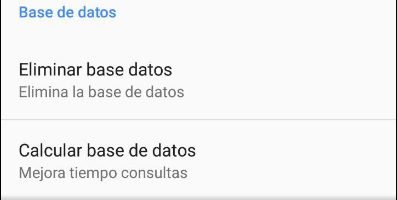
\includegraphics[scale=0.5]{imagenes/ajustesbd.png}  %el parámetro scale permite agrandar o achicar la imagen. En el nombre de archivo puede especificar directorios
\label{ajustesbd.png}
\caption{Pantalla ajustes. Sección base de datos}
\end{figure}

\section{Adicional}

En esta sección el usuario puede encontrar información relacionada con el proyecto, así como sobre su desarrollador. Al pulsar en cualquier opción esta le llevará a su correspondiente página web con una mayor cantidad de información.\\

Debido a que este tipo de sistema, \textit{CBIR}, no es muy conocido por los usuarios, al igual que los descriptores, se proporciona una serie de enlaces con información básica sobre ellos, en caso de que el usuario quiera aprender más o sienta curiosidad sobre el tema.

\begin{figure}[H] %con el [H] le obligamos a situar aquí la figura
\centering
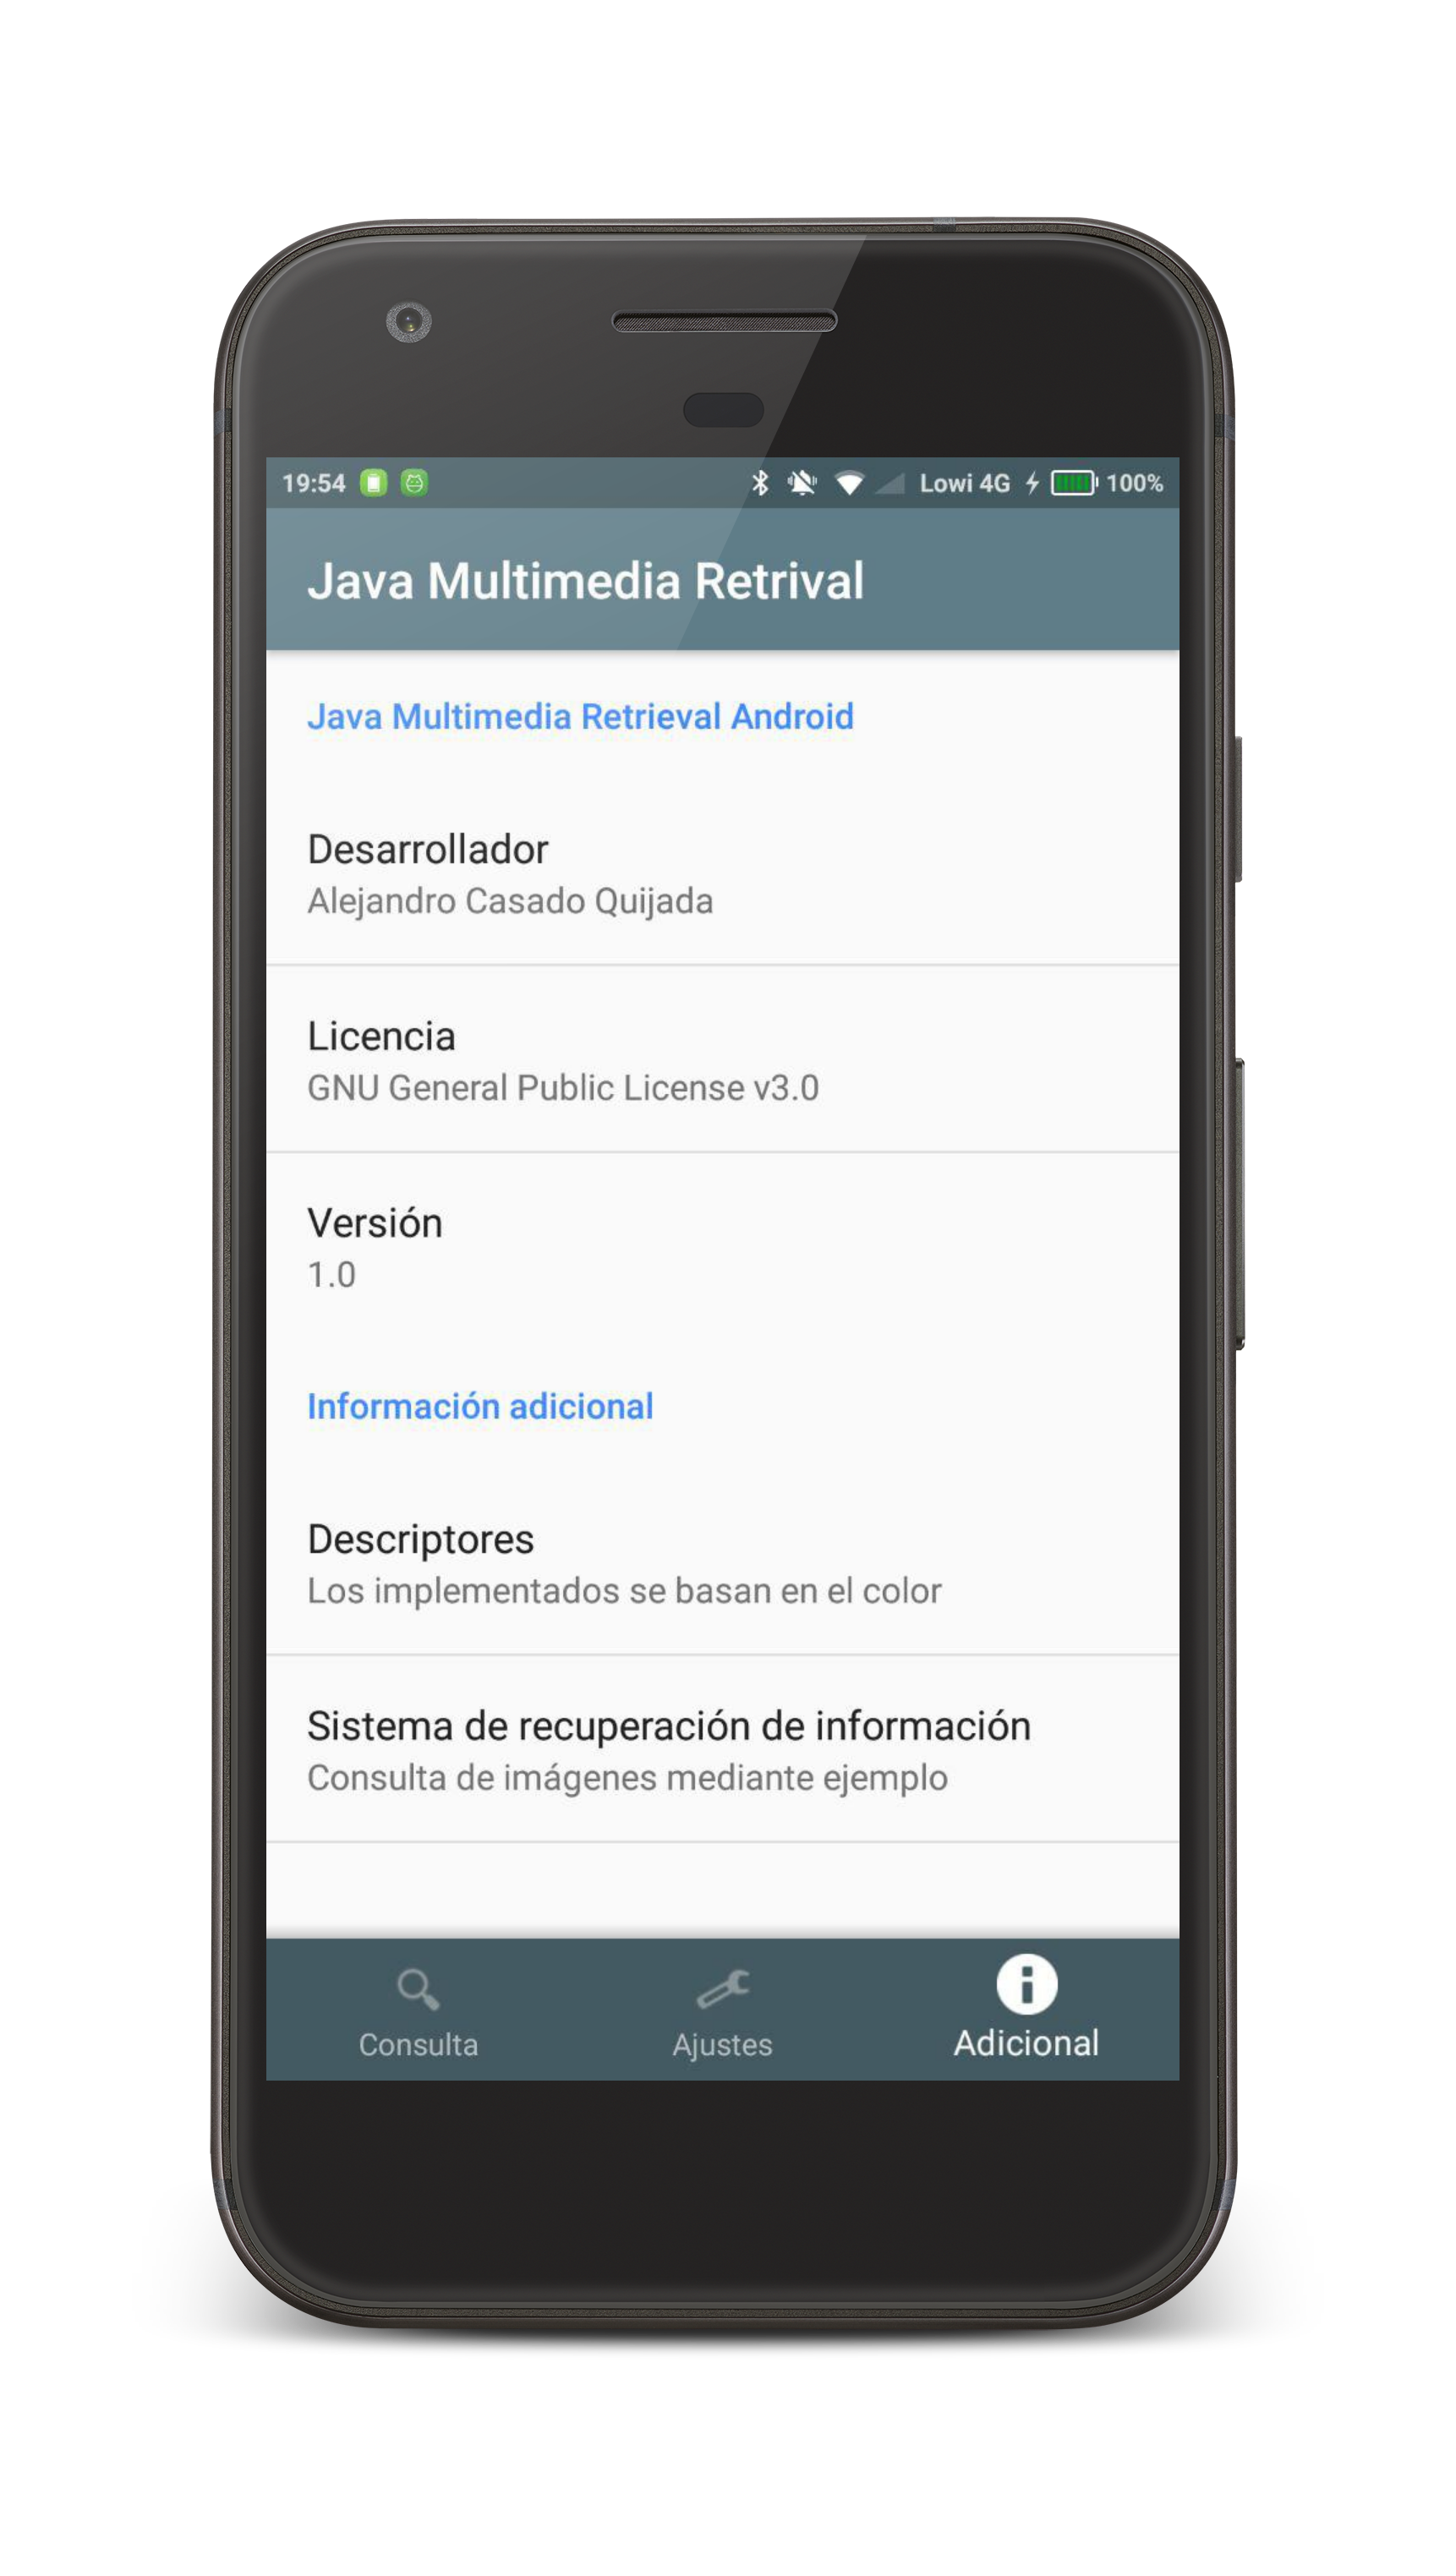
\includegraphics[scale=0.15]{imagenes/adicional.png}  %el parámetro scale permite agrandar o achicar la imagen. En el nombre de archivo puede especificar directorios
\label{adicional.png}
\caption{Pantalla adicional}
\end{figure}








